\section{Teori}
\subsection{Hvorfor Overvåke}
Nesten alle bedrifter i dag bruker IT-systemer for å gjøre bedriften mer effektiv og konkurransedyktig i dagens marked. Mange av disse systemene blir ofte tatt for gitt, fordi de rett og slett bare fungerer. Men hva skjer om e-posten en dag ikke virker, eller månedens lønn ikke kommer når den skal? I slike tilfeller kan en overvåkningsløsning være viktig for å oppdage og identifisere problemet tidlig.

Der en har avtaler knyttet til IT-tjenestene som blir levert kan et overvåkningssystem være med på å dokumentere at tjenestene har vært i henhold til SLA. Overvåkning kan også bidra til et bedre bilde av hvor pålitelige systemer og utstyr er, og kan hjelpe til med å kartlegge hvor systemene er sårbare. Dette kan igjen benyttes ved kapasistetsplanlegging. For de ansatte ved en driftsavdeling kan det også skape en trygghetsfølelse at det er noe som sjekker systemer, og gir beskjed om noe er galt.

Når en leverer tjenester innenfor IT er det viktig at det ikke er kunden som varsler om feilen, da har man allerede mistet kontrollen, og kundene ender opp som overvåkningsmekanismen. Her må kriteriene for varsling være finjustert, slik at en kan reagere før systemene krasjer.

I “The Practice of System and Network Administration” sier forfatteren det godt: \quote{you aren’t monitoring it, you aren’t managing it}.

\subsection{Generelt om overvåkning}
Overvåkning deles ofte inn i de to kategoriene historisk overvåkning og sanntidsovervåkning \cite{Practice of System and network adm.}. 

Ved historisk overvåkning blir data samlet inn for å ha statistikk over oppetid, ytelse og bruk. Ut fra disse dataene vil en kunne dra konklusjoner som for eksempel at VPN-tjenesten har hatt en oppetid på 99,9 \% over det siste året og gjennomsnittlig antall brukere har vært 100, med en økning på 10 \% den siste måneden. Dermed kan en få et overblikk over hvor lang nedetid en har hatt, og en har dokumentasjon på hvordan leveransen har vært opp mot avtalt leveranse.

Ved å se på stigningstallet kan en også forsøke å si noe om trenden og forventet fremtidig nivå som kan gi en indikasjon på nødvendige skaleringstiltak. For eksempel at en med dagens bruk av toner på kopimaskinen, vil den være tom innen fredag. 

Sanntidsovervåkning vil si at en sjekker tilstanden til en enhet eller tjeneste i et gitt intervall og så fort noe avviker fra normalen sendes det ut varlser. Målet her er at IKT-avdelingen skal kunne vite om noe er feil så fort som mulig, og helst før brukerne.

Den enkleste formen for overvåkning av en server er å sende en ICMP echo request (ping) og se om man får et svar (også kjent som pong). En måler tiden til en får et svar tilbake og sjekker hvor mange prosent av antallet forsøk man får svar på. Dette forteller deg om enheten du kontakter har en delvis fungerende IP-stack og om linjen i mellom er fungerende, men det forteller deg ikke noe om tjenestene som kjører. Det er tross alt tjenestene som kjører på enheten som er grunnen til at man trenger enheten i utgangspunktet.

En bedre løsning er å teste hver av tjenstene. For en webserver kan det være å prøve å hente ned forsiden av hjemmesiden som skal leveres og sjekke at man får reponsen “HTTP OK 200”. Da vil en vite at webserveren kjører og leverer ut sider riktig. Et skritt videre kan være å sjekke at siden inneholder riktig informasjon og at en ikke har blitt utsatt for f.eks en “defacing”.

\subsection{Overvåkning i ITIL}
ITIL (Information Technology Infrastucture Library) er et sett med standarder og konsepter som beskriver hvordan IT-tjenester kan kvalitetsikres innenfor leveranse, drift og support. ITIL er i dag i bruk i IT-bedrifter over hele verden og gir et felles rammeverk for hvordan en opererer innen IT-sektoren. ITIL blir definert i et sett med bøker som blir utgitt av Office of Government Commerce i Storbritannia.

Innenfor ITIL er prossessflyt og involvering av ulike prosesser ved hendelser essensielt.  Overvåkning av systemer og infrastruktur bak forretningskritiske systemer, og overvåkning av forretningskritiske systemer i seg selv er viktig i ITIL-prosessen Service Operations. Overvåkning og varsling er et viktig ledd for kunne å registrere en hendelse som kan være et engangstilfelle, eller en indikasjon på et underliggende problem. 

Forskjellen i ITIL på et problem og en hendelse er at hendelser kan gi indikasjon på et underliggende problem eller føre til at et problem oppstår. Når en hendelse inntreffer, enten ved at en bruker melder inn feil eller overvåkningsløsningen varsler om feil som har oppstått, vil servicedesk være første instans som må reagere. Servicdesk er derfor et viktig ledd for å opprettholde forretningskritisk funksjonalitet, og en god statusvisning og tilrettelagt varsling vil bidra til å identifisere problem.

Overvåkning er også en del av komponenten “Capacity Management” innenfor kategorien “Service Delivery”, som legger retningslinjer for proaktive handlinger framfor reaktive. Proaktive handlinger innebærer å være i forkant av hendelser som kan oppstå, og ikke å reagere når det allerede har skjedd; reaktivt. Informasjon fra overvåkningen kan hjelpe til med å identfisere situasjoner som kan håndteres før hendelser inntreffer og får innvirkning for brukere.

/ref http://www.teamquest.com/solutions/itil/service-support/
/ref http://www.itilfoundations.com/processes/capacity-management/
/ref http://apmdigest.com/event-management-reactive-proactive-or-predictive

\subsection{Hvilke Overvåkingsløsninger finnes}
Det finnes i dag mange løsninger for overvåkning av IT-systemer og infrastruktur /cite{http://en.wikipedia.org/wiki/Comparison\_of\_network\_monitoring\_systems}. Det ble tatt utgangspunkt prosjektets rammer og krav til fuksjonalitet, og plukket ut noen løsninger som ble sett nærmere på. Punktene om ønsket funksjonalitet ble også vektlagt slik at skulle være lettere å implementere dette i senere faser av prosjektetet eller senere prosjekter. 

Det ble også gjort en gjennomgang med oppdragsgiver og med diskusjon rundt de ulike løsningene. De som ble vurdert nærmere etter den første runden med research har alle en open source lisens og en utbredt brukermasse. 

Zenoss, har en open source-lisens på Zenoss Core. Zenoss brukes av mange store aktører /cite{http://www.zenoss.com/customers/index}, som gjorde denne til en verdig kandidat. Det ble likevel valgt å ikke bruke Zenoss på grunn av vinklingen de har mot “Enterprise Solutions” /cite{http://wiki.zenoss.org/Category:ZenPacks}, som involverer at man må kjøpe tilleggsmoduler til selve kjernen for å oppnå en fullverdig overvåkningsløsning.

Observium har lagt mye vekt på å visualisere ytelsesdata. Dette vises med statistikk og grafer over hver enhet som overvåkes. Observium er ikke ment for å erstatte en såkalt “UP/Down overvåkning”, da alarmer og grenseverdier for tjenester og servere ikke støttes. /cite{http://www.observium.org/wiki/Main\_Page}. Dette gjør at Observium ikke kunne benyttes i denne oppgaven.
Zabbix /cite{http://www.zabbix.com/index.php} var en av de sterkeste kandidatene. Denne støtter mange punkter som vi er ute etter, men antall plugins utenfor selve programvaren er for få. Zabbix er også et mer monolitisk system, og ikke like modulært. Dette er veklagt i oppgavebeskrivelsen /cite{http://knowledge.oscc.org.my/practice-areas/rnd/benchmark-report/comparison-report-on-network-monitoring-system/at\_download/file}

Nagios er kjent som en av de mest utprøvde overvåkningsløsningene /cite{http://en.wikipedia.org/wiki/Nagios, http://www.linux.org/article/view/the-monitoring-setup-part-1-installing-centreon-nagios-ndoutils, http://www.cio.com.au/article/373428/5\_open\_source\_network\_management\_projects\_watch/}

/cite{http://sectools.org/tag/traffic-monitors/}, og har et enormt antall brukere som aktivt bidrar til å utvikle plugins og moduler til Nagios-kjernen /cite{http://nagios.org/about/community}. Det finnes flere websider der brukere bidrar med og diskuterer plugin-er og moduler, blant annet Nagios Exchange (http://exchange.nagios.org) og Monitoring Exchange (https://www.monitoringexchange.org). Det som gjør Nagios spesielt interessant er fleksibiliteten Nagios har med tanke på konfigurasjon, integrasjon og plugin-er.

Icinga er en fork av Nagios, og har blitt utviklet videre siden 2004. Konfigurasjon, plugin-er og addons er kompatible med det som benyttes for Nagios. Forskjellen er selve arkitekturen som er nå består tre separate deler, og abstraksjon mot databaselaget. 

I Figur \ref{losninger} vises en oversikt over hvor ofte hver av disse har blitt benyttet i et Google-søk i perioden januar 2008 - januar 2013. Hentet fra Google trends.

\begin{center}
\begin{figure}
    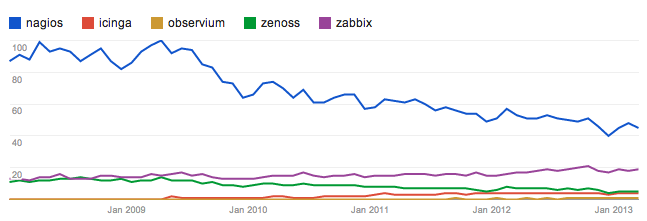
\includegraphics{img/monitoring_google_trends}
    \caption{Google Trends: Monitoring}
    \label{losninger}
\end{figure}
\end{center}

\subsection{Valg av kjerneprogramvare}
Valg av kjerneprogramvare var gruppens viktigste valg, da det la grunnmuren for restenu av prosjektet, og ville få stor innvirkning på sluttresultatet. Etter en vurdering av alternativene som nevnt over ble det besluttet å bygge overvåkningsløsningen på Icinga framfor nagios.

Icinga sitt distribuerte system består av kjernen, som står for prossessering, et databaselag, og administrering av systemet via et webgrensesnitt. Dette er tilrettelagt for et distribuert oppsett. Nagios sin arkitektur har avhengigheter mellom web og lagring av status, som fører til at disse ikke kan separeres. Det er derimot mulig å separere MySQL-databasen som Nagios benytter. /ref https://www.icinga.org/about/architecture/

For uthenting av informasjon i Icinga er det utviklet et API som brukes via Icinga-Web. Dette gir ett punkt for uthenting av data, med samme oppbygging for alle spørringer. I Nagios er det ikke noen standardisert måte å hente ut informasjon. /ref http://docs.icinga.org/latest/en/icinga-web-api.html

Et annet punkt er støtte for LDAP-autentisering integrert i Icinga Web, som videre kan benyttes til å styre aksess til ulik informasjon for brukere. Med Nagios kan en også innføre LDAP-støtte, men dette blir da autentisering via en web-server, og videre kontroll av aksess er ikke mulig. Nagios har noe aksessyring, men det er bare på et objekt kalt Contact-groups. Her har icinga aksesstyring på en rekke flere objekter. /ref https://www.icinga.org/about/icingaweb/

For databaseoppsett støtter Icinga de tre databasemotorene PostgresSQL, Oracle og MySQL, i motsetning til Nagios som bare har støtte for MySQL. I oppgavebeskrivelsen er det krav om MySQL, men for fremtidig bruk av Icinga er det mulighet for å benyttet de to andre.

(http://www.freesoftwaremagazine.com/articles/nagios\_and\_icinga)

https://www.icinga.org/nagios/

\subsection{Icinga}

For å kunne forstå implementasjonsdelen av prosjektrapporten behøves noe innsikt i hvordan Icinga fungerer. I dette delkapittelet er det viktigste forklart.

\subsubsection{Arkitektur}

Icinga består som i vist i Figur \ref{icingacomponents} av tre separate komponenter som sammen danner en overvåkningsløsning.

\begin{center}
\begin{figure}
    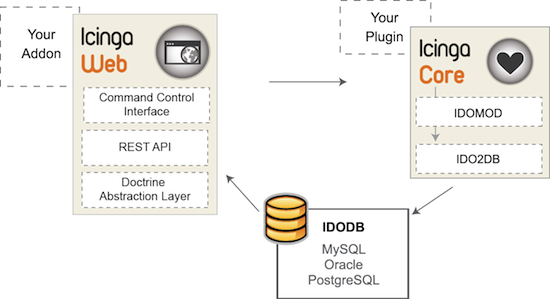
\includegraphics{img/icinga_architecture}
    \caption{Icingas tre komponenter}
    \label{losninger}
\end{figure}
\end{center}

\paragraph{Core}
Icinga Core håndterer planlegging av sjekker gjennom plugins og tar i mot resultatene av disse. Denne informasjonen sendes gjennom SSL-krypterte TCP-sockets videre til IDO2DB-prosessen (Icinga Data Out to Database) gjennom et interface kalt IDOMOD (Icinga Data Out Module). Ved å bruke disse abstraksjonslagene kan databasemotoren enkelt byttes ut. I dokumentasjonen er det laget veiledninger for MySQL, PostgreSQL og Oracle.
https://www.icinga.org/about/architecture/

IDOMOD og IDO2DB kommer i en samlet pakke (IDOutils), men kan separeres ut for å skape et distribuert oppsett. CERN i Sveits har nylig implementert et et slikt oppsett med hjelp av lastbalansereren “modgearman”. (http://accelconf.web.cern.ch/accelconf/icalepcs2011/papers/wepmu035.pdf)

\paragraph{Web}

I utgangspunktet kommer ikke Icinga med noe webgrensesnitt. Men det er mulig å installere to forskjellige pakker for å få dette. I begge kan en få en oversikt over tilstanden til hosts og services, se konfigurasjon og utsendte varsler, samt utføre kommandoer.

Icinga Classic baserer seg på det samme vindu-oppsettet som Nagios. For uthenting av data benyttes CGI-moduler.

Icinga-web er en total omskrivning av webgrensesnittet. Det er Ajax-drevet, Web 2.0-inspirert front-end, som har flere lag mellom kjernen av Icinga og visningene:

\begin{itemize}
	\item Doctrine Abstraction Layer henter informasjon fra databasen. Det kan også benyttes av utviklere for å legge til egne moduler i Icinga-Web med uthenting av informasjon fra andre databaser.
	\item REST API presenterer dataene fra DAL til Icinga Web. Her kan autentisering utføres slik at en kan sette hvilken informasjon ulike brukere skal kunne se.
	\item Command Control Interface utfører kommandoer.
\end{itemize}

\subsection{Objekter}
All konfigurasjon av Icinga gjøres i rene tekstfiler. I selve konfigurasjonsfilen icinga.cfg settes banen til der konfigurasjonsfilene finnes. Icinga vil da ved oppstart lete rekursivt gjennom mappen etter filer som ender med “.cfg”.

Konfigurasjonsdataene er bygget rundt det som i Icinga kalles objekter. Dette er en samling av konfigurasjon som hører sammen. Selv om en ikke kan si at Icingas objekter er det samme som objekter i programmeringsverden, benyttes mange av de samme begrepene og konseptene.

En rekke objekter er definert i Icinga, som vist i Tabell \ref{objekter}.

\begin{changemargin}{-1cm}{-1cm}
\begin{table}
\begin{center}
%\begin{tabular}{|p{2.0in}|c|c|c|} \hline
\begin{tabular}{ | p{3.5cm} | p{6.5cm} | p{6cm} |} \hline
	\textbf{Objekt} & \textbf{Forklaring} & \textbf{Eksempel} \\ \hline
	Host & En enhet med en addresse (typisk IP-adresse eller mac-adresse). & Server, switch, router etc. \\ \hline
	Command & En kommando som skal kjøres på overvåkningsserveren & Et program, f.eks check\_ping. \\ \hline 
	Service & Kombinasjonen av en host og en kommando. Det er dette som overvåkes. & Sjekk oppetid: kommandoen “check\_uptime” skal kjøres på “dc1”. \\ \hline
	Servicegroup & Servicer knyttet til hoster satt sammen til en “Applikasjon”. & En applikasjon har tre prosesser som må være kjørende for at applikasjonen fungerer. Her grupperer vi disse og får et helhetsbilde. \\ \hline
	Contact & Når og hvordan en person skal kontaktes anngående en service. & Jens skal få en SMS hvis DHCP ikke er tilgjengelig. \\ \hline
	Timeperiod & Navn og definisjon av en tidsperiode. & Mellom 08.00 og 16.00 på annenhver tirsdag, hvis det er den tredje dagen i måneden. \\ \hline
	Host dependency & En eller flere avhengigheter. Dersom en en host er avhengig av en annen, og den andre går ned trenger en ikke prøve å utføre sjekker på denne. & kantswitch1 er avhengig av kjerneswitch. \\ \hline
	Service dependency & Samme som host, men for service. & Captive portal er avhengig av RADIUS. \\ \hline
	Host escalation & Hva skal skje etter at en host har vært nede etter en definert tid. &	Om dc1 har vært nede i 30 minutter, send e-post til Ola Sysadmin. Etter 60 minutter send SMS til alle i admin contactgroup-en \\ \hline
	Service escalation & Samme som for host, men for tjenester. & Om DNS har vært nede i 30 minutter, send e-post til Kari Sysadmin. Etter 60 minutter send SMS til alle i admin hostgroup-en. \\ \hline
	\end{tabular}
	\caption{Oversikt over objekter i Icinga}
	\label{objekter}
\end{center}
\end{table}
\end{changemargin}

I tillegg til disse kan host, service og contact grupperes med henholdsvis hostgroup, servicegroup og contactgroup.

Det er også to objekter med metainformasjon, “hostextinfo” og “serviceextinfo” der en kan definere ekstra konfigurasjon som bildebaner, notater og koordinater for hosts og services.

Den siste objekttypen er module. Her spesifiseres konfigurasjon for en modul som utvider funksjonalitet i Icinga-Web.

Sammenhengen mellom objektene er viktig å forstå for å skjønne hvordan sjekker utføres i Icinga. I et serviceobjekt defineres hvilket command-objekt som skal benyttes for å teste tjenesten og hvilke host eller hostgroup dette skal sjekkes på. Dette er vist i Figur \ref{command_host_service}

\begin{center}
\begin{figure}
    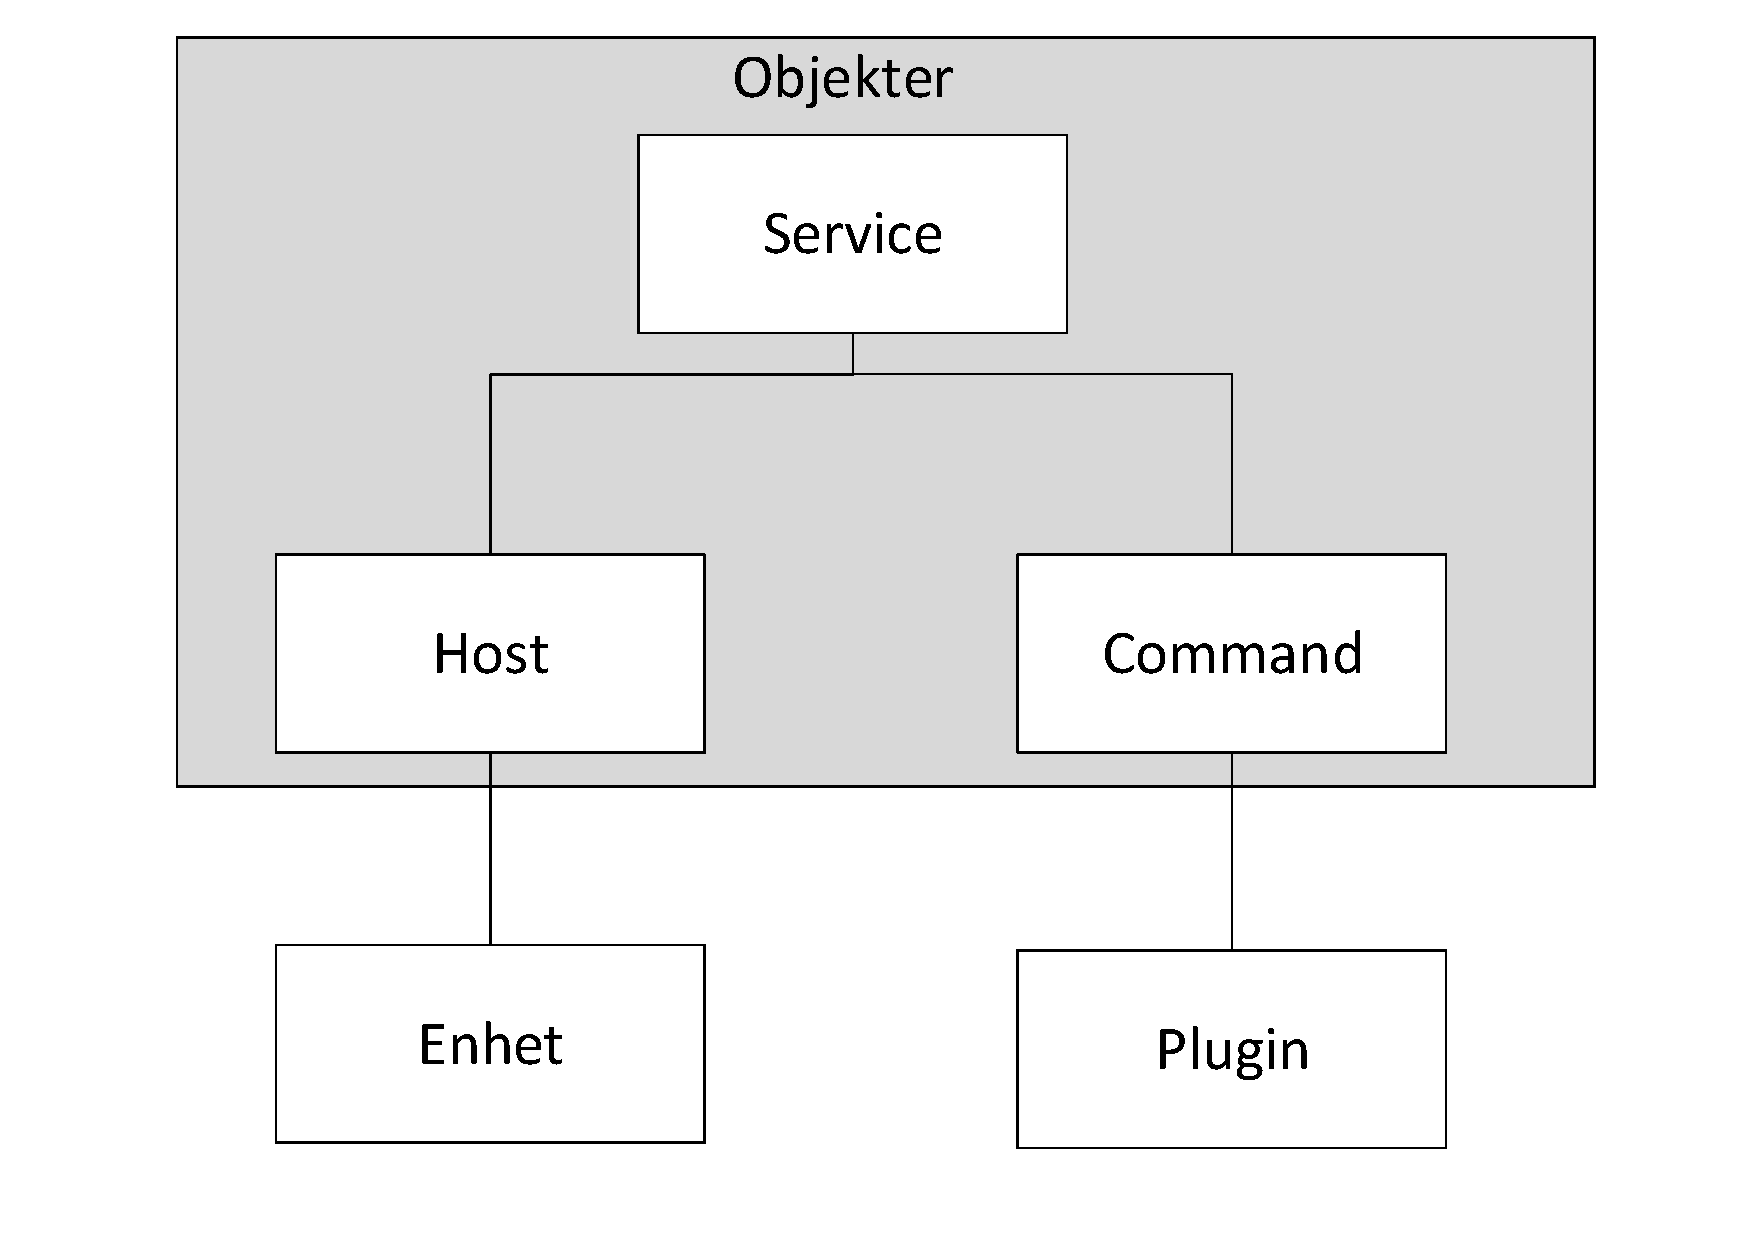
\includegraphics{img/command_host_service}
    \caption{Sammenhengen mellom host service og command objekt.}
    \label{losninger}
\end{figure}
\end{center}

\subsection{Plugins}
Icinga i seg selv kommer uten noen overvåkningssjekker. Til dette benyttes plugins.

Plugins i Icinga er eksterne programmer som kjøres der outputen hentes inn som data. Resultatet av sjekken hentes fra exit-koden (http://en.wikipedia.org/wiki/Exit\_code) og oversettes til en state etter Tabell \ref{state}.


\begin{table}
	\begin{center}
	\begin{threeparttable}
	\begin{tabular}{ | l | l | l |} \hline
    \textbf{Plugin Return Code} & \textbf{Service State} & \textbf{Host State} \\ \hline
	0 & OK & UP \\ \hline
	1 & WARNING & UP or DOWN/UNREACHABLE* \\ \hline
	2 & CRITICAL & DOWN/UNREACHABLE \\ \hline
	3 & UNKNOWN & DOWN/UNREACHABLE \\ \hline

	\end{tabular}
	\begin{tablenotes}
	\small
	\item *Ved bruk av Aggressive host checking. (cite http://docs.icinga.org/1.8/en/pluginapi.html).
	\end{tablenotes}
	\caption{State oversikt}
	\label{state}
	\end{threeparttable}
	\end{center}
\end{table}

\subsection{Sjekker}
Staten for en service eller en host vil bestemmes ut i fra et returnert resultat av en aktiv eller passiv sjekk, forskjellen på disse to vil bli forklart i de neste delkapitlene.

Dersom en aktiv eller passiv sjekk resulterer i en annen state enn “OK” er det to typer av state-en, “soft” og “hard”. Første gang en plugin returnerer en feil vil staten bli satt til “soft” i tillegg til service- eller host-staten. Etter dette vil sjekken kjøres hyppigere for å sjekke om det er snakk om et forbigående problem. Etter et satt antall ganger der pluginen fortsatt ikke returnerer “OK”, vil staten skifte til “hard” og det sendes ut varslingsmelding /ref {varslingsmelding}.

\subsubsection{Aktive sjekker}
En aktiv sjekk defineres ut i fra et command-objekt med parametere og et tidsintervall i service- og host-objekter. I command-objektet defineres en plugin som skal kjøre og returverdien vil bestemme hvilken state service- eller host-objekter har. 

\begin{center}
\begin{figure}
    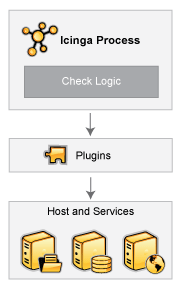
\includegraphics{img/activechecks.png}
    \caption{Aktive Sjekker}
    \label{active_checks}
\end{figure}
\end{center}

\subsubsection{Passive sjekker}
Passive sjekker går motsatt vei av av en aktiv sjekk. Her vil hver host si ifra når verdier har overgått en satt grense eller en feil har oppstått. Dette gjøres ved at et eksternt program skriver en linje med informasjon om tjenesten og sjekkresultat til en fil som Icinga sjekker periodisk.

Fordelen er at en får beskjed med en gang noe er galt og kan gi en raskere varsel. Det vil også avlaste Icinga-serveren da alle sjekker utelukkende vil bli kjørt lokalt. En vil da måtte åpne for at kommunikasjon kan initieres fra alle enheter som skal overvåkes til Icinga-serveren. Men en mister samtidig muligheten til å samle all konfigurasjon på ett sted \ref{passive_checks}.

\begin{center}
\begin{figure}
    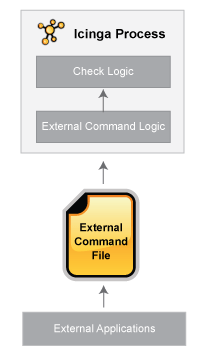
\includegraphics{img/passivechecks.png}
    \caption{Passive Sjekker}
    \label{passive_checks}
\end{figure}
\end{center}

\subsubsection{Hostsjekk}

Resultatet av en host-sjekk vil avgjøre om en host er i state “UP” eller “DOWN”. 

Det er ikke et fast tidsintervall for en hostsjekk [d]med mindre check\_interval er definert. Icinga vil kjøre denne sjekken om en service som er satt opp for host-en skifter state. Servicer som er definert for en host som er i “DOWN” vil automatisk bli satt som “ Known service problems”, og ingen sjekker vil bli kjørt på dem før host-en er “OK” igjen.

Grunnsjekken for en host defineres i host-konfigurasjonen med “check\_command”.

\begin{lstlisting}
define host {
	...
	check_command                   check_host_alive
}
\end{lstlisting}

\paragraph{Variabler}
For å kunne gjøre konfigurasjon av Icinga mest mulig dynamisk er det en rekke forhåndsdefinerte variabler en kan bruke i konfigurasjonsfilene. Disse kalles makroer. En fullstendig liste over disse og hvor de kan benyttes finnes i Icinga-dokumentasjonen. /ref http://docs.icinga.org/latest/en/macrolist.html $HOSTADDRESS$ kan for eksempel benyttes i et command-objekt slik at den bare må skrives en gang, og ikke for hver host. En kan også definere egne variabler som f.eks “\_SSHPORT”. Disse kan også sendes videre til selve kommandoen som kjøres og benyttes som argumenter til programmet som kjører en sjekk, slik:

\begin{lstlisting}
define host {
	host_name	example_server
	_SSHPORT	222
}
define command {
	command_name	check_ssh
	command_line	$USER1$/check_ssh -H $HOSTADDRESS$ -p $_HOSTSSHPORT$
}
\end{lstlisting}

Her benyttes de innebygde variablene “USER1” for banen til pluginen som kjøres, “HOSTADDRESS” for IP-en til den hosten som sjekken skal kjøres på og den egendefinerte variabelen “\_SSHPORT” som defineres på hosten.

\paragraph{Templates}

En template er ikke et objekt i seg selv, men en mal for et objekt. Med direktivet “register 0” vil ikke Icinga registrere dette som noe som skal overvåkes. Ved å bruke direktivet “use” kan en i et annet objekt “arve” konfigurasjonen fra templaten. Templates kan også arve, og en kan dermed sette opp et hierarki der en spesifiserer generell konfigurasjon og arver nedover til mer spesiell. 

I eksempelet under er generell konfigurasjon for alle hosts definert i “generic\_host”, som brukes i de andre objektene. I “generic\_firewall” erstattes verdien for kontaktgruppe, og i cisco\_firewall settes en egendefinert variabel:

Template-en generic\_host: 

\begin{lstlisting}
define host {
	name                            generic_host    ; The name of this host template
	notifications_enabled           1       ; Host notifications are enabled
	event_handler_enabled           1       ; Host event handler is enabled
	flap_detection_enabled          1       ; Flap detection is enabled
	failure_prediction_enabled      1       ; Failure prediction is enabled
	process_perf_data               1       ; Process performance data
	retain_status_information       1       ; Keep status after Icinga restart
	retain_nonstatus_information    1       ; Keep non-status after Icinga restart
	check_command                   check-host-alive
	max_check_attempts              10
	normal_check_interval           5
	retry_check_interval            2
	notification_interval           0
	notification_period             24x7
	notification_options            d,u,r
	contacts                nils
	contact_groups                  all_contacts
	register                        0       ; Not a real host, just a template
}
\end{lstlisting}

Template-en generic\_firewall:

\begin{lstlisting}
define host {
   name             generic_firewall
   use              generic_host
   contact_groups        firewall_admins
   register         0
}
\end{lstlisting}

Template-en cisco\_firewall (arver i fra generic\_firewall):

\begin{lstlisting}
define host {
        name                cisco_firewall
        use                generic_firewall
        register        0
        _WANPORT        WAN ; Custom variable for WAN port to monitor
}
\end{lstlisting}

Host-objektet hig-hw1 (arver i fra cisco\_firewall):

\begin{lstlisting}
define host {
        host_name        hig-fw1
        use                cisco_firewall
}
\end{lstlisting}

\subsubsection{Regulære uttrykk}
%Ved å sette “use regular expressions” i konfigurasjonen for Icinga, kan en benytte regulære uttrykk i attributter i et objekt, der en refererer til andre objekter. Icinga vil automatisk tolke navnet som et regulært uttrykk dersom det inneholder ‘*’, ‘?’, ‘+’, eller ’\’.

Dette kan være nyttig dersom en for eksempel vil legge alle hoster i en hostgroup, som har en navnekonvensjon som gjør at hver av hostene unikt kan identifiseres ved å bytte ut deler av navnet med en variabel.

%I eksempelet nedenfor brukes det regulære uttrykket “\^HiG\[0-9\]+\$” i attributten “members” til å legge til alle konfgurerte hosts der navnet starter på “HiG” etterfulgt og avsluttet med ett eller flere siffer mellom 0 og 9, i hostgroup-objektet “all\_servers”.

\begin{lstlisting}
define hostgroup {
	hostgroup_name          all_servers
	alias                        All Servers
	members                ^HiG[0-9]+$
}
\end{lstlisting}

Det kan også være nyttig for å ekskludere en host fra en servicesjekk som den ellers skulle kjørt. I eksemplet nednfor er HiG3 medlem av hostgroup-en “windows-servers”, men blir ekskludert fra å kjøre sjekken på diskplass ved å sette “!HiG3”:

\begin{lstlisting}
define service {
service_description        Disk space
hostgroup_name        windows_servers
host_name                !HiG3
check_command        win_nrpe!CheckDriveSize!Drive="C" MaxWarnUsed=80% MaxCritUsed=90%
use                generic_service
}
\end{lstlisting}

\subsection{Avhengigheter}

I Icinga kan man definere de tre ulike typene avhengigheter “Parent”, “Service dependency”, “Host dependency“. Disse har innvirkning på hvilke varsler som sendes ut og statusen de ulike service-ene og host-ene får. Alle er definert som egne objekttyper og krever egen konfigurasjon. 

\subsection{Parent}
Et host-objekt kan settes som en “parent” til et annet host-objekt. Host-objekter som har et parent blir betegnet som en child-host eller child-service. Dette brukes primært for å unngå varsler om alle hosts som har en gitt host som parent om denne går ned. For eksempel hvis kjernerouteren går ned, ønskes ikke varsler for eventuelle host-er som har denne som parent. Disse vil ikke lengre bli sjekket og blir markert som “UNREACHABLE”. Tjenester som tilhører host-ene vil bli markert som “UNKNOWN”.

For redundante oppsett kan et host-objekt ha flere “parents” definert. Host-objektet vil da være UP så lenge en “parent”-host er UP.

Ut ifra “parent”-relasjonene mellom host-objekter i konfigurasjonsfilene genereres også et “Status Map” over nettverket, som vist i Figur /ref{statusmap}. Dette brukes til å visualisere alle relasjonene, og vil gjengi redundante oppsett og hvilke host-objekter som er påvirket av at “parent”-hosten er DOWN.

\subsection{Service dependency}

Service dependency er en egen objekttype der en kan sette opp avhengighet mellom to service-er. Formålet med dette er å unngå varsel hvis en tjeneste går til DOWN, som følge av at en annen tjeneste er nede. For eksempel bør det ikke varsles at tjenester som er avhengig av autentisering via LDAP-serveren får “access denied”-feilmeldinger, hvis LDAP-serveren er DOWN. 

Icinga sjekker om avhengigheter er definert for en service-sjekk, før denne utføres. Dette er med på å bestemme om det blir sendt ut varsel for service-en.

I eksempelet under er tjenesten “Check SMB” på HiG3 avhengig av master tjenesten Check LDAP på HiG3. “execution\_failure\_criteria” bestemmer ved hvilke tilfeller tjenesten ikke skal sjekkes. Her er den satt til ‘c’, som vil si at Check SMB skal ikke kjøres dersom Check LDAP er i “critical” tilstand.

\begin{lstlisting}
define servicedependency {
	host_name                                         HiG3
	service_description                         Check LDAP
	dependent_host_name                         HiG3
	dependent_service_description         Check SMB
	execution_failure_criteria         c
	notification_failure_criteria         c
}
\end{lstlisting}

Ved standard konfigurasjon vil Icinga benytte siste hard state for master services. Det vil si at hvis denne er satt til 4 retries vil ikke Check SMB stoppes fra å kjøres før Check LDAP har blitt sjekket 4 ganger. 

På attributten notification\_failure\_criteria kan det settes hvilke service-state-er en ikke skal varsle for. Dette er hovedgrunnen til at det settes opp slike avhengigheter. Når denne er satt til ‘c’ vil skale det ikke varsles om master-servicen går til critical state.

Service-objekt har også muligheten til å arve avhengighetene til master-service ved å sette direktivet inherits\_parent 1. Da vil for eksempel Check SMB arve fra service-objektet som Check LDAP arver fra.

For å konfigurere avhengigheter mellom tjenester som kjører på samme host kan en utelate “dependent\_host\_name”. Dette er benyttet i oppsettet for å sette opp en avhengighet mellom NRPE-tjenesten og alle sjekker som går via NRPE.

\begin{lstlisting}
define servicedependency{
#       dependent_host_name   ; Not defined to make dependancy on same host            
        hostgroup_name           linux_servers
        service_description         NRPE-daemon
        dependent_service_description   NRPE Check *
        execution_failure_criteria      c
        notification_failure_criteria   c
}
\end{lstlisting}

En kan også erstatte host\_name og dependant\_host\_name med hostgroup og dependant\_host\_group for å lage avhengigheter på alle hoster som tilhører gruppa.

\subsection{Host dependency}

For å sette en avhengighet mellom to host-er benyttes “host dependency”. Dette må ikke forveksles med “parent”, som refererer til nettverksoppsettet. Mens en host dependency går på at en host er avhengig av en annen. Host dependency er bare nyttig i veldig spesielle tilfeller, da det for de fleste tilfeller vil det være avhengigheter til en eller flere tjenester på hosten. 

her er det anbefalt å bruke parents i stedet. /cite Nagios-boka og http://docs.icinga.org/latest/en/dependencies.html.

\subsection{Protokoller og agenter }
For å kjøre sjekker på enheter må Icinga-serveren kunne kommunisere med operativsystemene på de ulike enhetene. Icinga henviser til protokollene SSH, SNMP, RPC (WMI) og agentene NRPE og NSCA (en del av pakken NSClient++). http://docs.icinga.org/1.8/en/ch09.html http://docs.icinga.org/1.8/en/ch10.html 

\subsubsection{NRPE}
NRPE (Nagios Remote Plugin Executor) består av en plugin (check\_nrpe) på icinga-servern og en daemon som installeres på hver server som skal overvåkes. NRPE eksekverer lokale plugins på den eksterne serveren og returner dataen fra denne til check\_nrpe. Tillatelse for eksekveringer defineres i en config-fil på hver server, der en oppgir hvilke IP-er som kan koble seg til og hvilke kommandoer som er gyldige. 

\begin{center}
\begin{figure}
    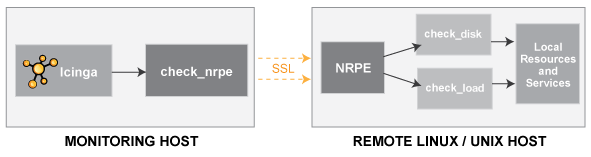
\includegraphics{img/nrpe.png}
    \caption{NRPE}
    \label{nrpe}
\end{figure}
\end{center}


\subsubsection{SSH (Secure Shell)}

Gjennom en tilkobling til en SSH-server kan en spesifisere en kommando som skal kjøres og ta outputen til det orginale shellet. Dette virket som den beste måten å overvåke Linux-servere ved starten av prosjektet. SSH-prosjektet er meget utbredt og blir aktivt sjekket for sikkerhetshull. SSH er også installert på de aller fleste Linux-servere, og man vil dermed unngå å lytte på en ekstra port. 

Ulempen med å kjøre sjekker over SSH er at man må sette opp nøkkelbasert innlogging mellom Icinga-serveren og alle Linux-serverne som skal overvåkes. En kan selvsagt begrense rettigheter for nagios-brukeren som kjører sjekkene, men den vil fortsatt ha muligheten til å logge inn til et shell og eksekvere kommandoer. Dette kan føre til at en potensiell angriper via Icinga-serveren har en vei inn til alle servere som overvåkes.

SSH gir også endel overhead[e] (ref man page) både på nettverkstrafikk og i CPU-tid. En måte å minske dette på er å benytte SSH med ControlMaster. Dette innebærer en endring i SSH-konfigurasjonen på serveren der SSH-klienten lagrer informasjon om hver utgående TCP- tilkobling slik at denne kan benyttes om nye tilkoblinger blir forsøkt mot samme host. Dermed unngår en å sette opp en ny TCP-tilkobling for hver ny sjekk som skal utføres på hosten.  

\subsubsection{SNMP (Simple Network Management Protocol)}

Det meste av mer avansert nettverksutstyr i dag støtter SNMP (/cite Douglas R. Mauro \& Kevin J. Schmidt. (2001). Essential SNMP (1st ed.). Sebastopol, CA: O’Reilly \& Associates). Gjennom protokollen SNMP har man en enkel og effektiv måte å overvåke på, samt en standard som leverandørene følger. 

SNMP baserer seg på variabler som blir gjort tilgjengelig på enheten som skal overvåkes (kalt agenten). Disse variablene er definert i en Management Information Base (MIB). MIB-filene er ofte tilgjengelige på produsentens hjemmeside. Her beskrives strukturen for dataen i et hiarkisk navnerom som inneholder Object Identifier (OID). Hver OID identifiserer en variabel som kan bli lest eller satt via SNMP. Enheten som ber om disse variablene kalles “manager”. 

En ulempe med SNMP er at OID-ene er lange og tunge å lese. For eksempel for å hente ut batterikapasiteten på en APC UPS benyttes OID-en:

1.3.6.1.4.1.318.1.1.1.2.2.1.0

Dette kan oversettes til:

iso(1). org(3). dod(6). internet(1). private(4). enterprises(1). apc(318). products(1). hardware(1). ups(1). upsBattery(2). upsAdvBattery(2) upsAdvBatteryCapacity.0

Denne OID-en er definert i APCs MIB-fil “PowerNet MIB”. Ved å laste inn denne kan en også benytte “PowerNet-MIB::upsAdvBatteryCapacity.0”.

SNMP finnes i flere versjoner. I dag brukes for det meste versjon 2c og den nyeste, versjon 3.[f] v2c og v1 er ikke kompatible, men i praksis støtter det meste av utstyr som har støtter v3 eller v2c og v1 (cite http://tools.ietf.org/html/rfc3584). Hovedforskjellen mellom versjon 2c og 3 er at versjon 3 krypterer dataene over nettverket, men krever da også mer konfigurasjon og vedlikehold. Sikkerhetsaspektet ved disse er diskutert videre i sikkerhets kapittelet /ref{sikkerhet}. 

Man har to muligheter når man skal overvåke med SNMP. Enten kan enhetene selv rapportere inn hendelelser via SNMP trap/inform, eller så kan serveren spørre enhetene via SNMP GetRequest. Valg av det første medfører at en kan gjøre varsling umiddelbart, men da må også hver enhet konfigureres med parametere for hvilke traps som skal sendes og hvor. Icinga har ingen støtte for å motta traps, men en kan installere en egen daemon for dette og rapportere inn data som passive sjekker. 

For å benytte SNMP trap/inform må en tillate tilkoblinger til overvåkingsserveren i stedet for bare fra. Hvilke trap meldinger som skal sendes må også konfigureres på hver enhet, og en vil da ikke kunne ha all konfigurasjon er på ett sted.

%\begin{center}
%\begin{figure}
%    \includegraphics{img/snmp.gif}
%    \caption{SNMP}
%    \label{SNMP}
%\end{figure}
%\end{center}

SNMP benytter seg av UDP for å levere traps. Fordi UDP er en såkalt upålitelig protokol, det vil si at det ikke er noen omsending av pakker eller noen tilbakemelding (ack) for at pakkene kommer fram. Derfor kan en risikere å miste en trap. SNMP inform, som kom i SNMPv3, løser dette ved at agenten vil sende en ny inform-pakke i et intervall, helt til manageren gir beskjed om at trap-en er mottatt.

[g]

For å benytte SNMP på Windows- og Linux-servere kreves installasjon av en SNMP-agent. http://technet.microsoft.com/en-us/library/bb726987.aspx http://www.net-snmp.org/ 

\subsubsection{WMI (Windows Management Instrumentation)}
WMI er et grensesnitt som gjør det mulig å lage programmer eller script som utfører oppgaver mot operativsystemet Windows, enten lokalt eller mot eksterne maskiner. Disse oppgavene kan være alt fra å restarte maskinen til å hente ut logger over hendelser som har intruffet på maskinen. I et overvåkningssytem vil det være mest relevant å kjøre kommandoer som henter ut informasjon om maskinen og tjenester som kjører på den. Dette kan for eksempel være hvilke prosesser som bruker mest CPU-tid.

For å benytte WMI-spørringer fra en ekstern enhet må det konfigureres brukertilgang og brannmurregler /cite http://msdn.microsoft.com/en-us/library/windows/desktop/aa822854(v=vs.85).aspx. Med NSclient[h]++ har en mulighet til å kjøre WMI-queries over NRPE.

\subsubsection{Valg av Agenter}
Valg av protokoll eller agenter har basert seg på følgende punkter:
\begin{itemize}
	\item Ressursbruk (CPU)
	\item Nettverkstrafikk
	\item Utrulling
	\item Sikkerhet
	\item Round-trip
\end{itemize}
Nettverkstrafikken som blir generert ved en enkelt NRPE- og SSH-sjekk ble målt ved å benytte et enkelt bash-script som kjørte en disk-sjekk 100 ganger. 

\begin{lstlisting}
#!/usr/bin/env bash
if [ "$1" == "ssh" ]; then
    cmd="/usr/lib/nagios/plugins/check_by_ssh -H 10.60.0.21 -C \"/usr/lib/nagios/plugins/check_disk -W 10% -C 5% -M -A\" > /dev/null"
elif [ "$1" == "nrpe" ]; then
    cmd="/usr/lib/nagios/plugins/check_nrpe -H 10.60.0.21 -c check_all_mounts -a 10,5 > /dev/null"
else
    echo "You must specify ssh or nrpe as the first argument"
    exit 1
fi
for i in {1..100}; do
    eval $cmd
done
exit 0
\end{lstlisting}

Både serveren og klienten stod i et eget nettverk i Virtualbox sammen med en Windows-maskin med et nettverkskort satt i promiscious mode, for å kunne sniffe nettverkstrafikken. Denne fanget nettverkstrafikken med WireShark. SSH-trafikken mellom de to maskinene ble hentet ut og data for hver “samtale” kunne analyseres.  

Analyse av hvor mye CPU-tid NRPE og SSH trenger for å utføre sjekker ble også gjennomført. Fordi hver sjekk går veldig raskt ble det kjørt 100 disksjekker, 100 ganger. Time-kommandoen ble brukt for å se på tiden brukt i user- og kernel-mode ved 100 sjekker. Dette ble gjort ved å bruke et bash-script som kjører scriptet i x.x.

\begin{lstlisting}
#!/usr/bin/env bash

args=(nrpe ssh)

for arg in "${args[@]}"; do

        for i in {1..100}; do

                /usr/bin/time -f "%U\t%S" run_check.sh $arg
        done
done
exit 0
\end{lstlisting}

\begin{center}
\begin{figure}
    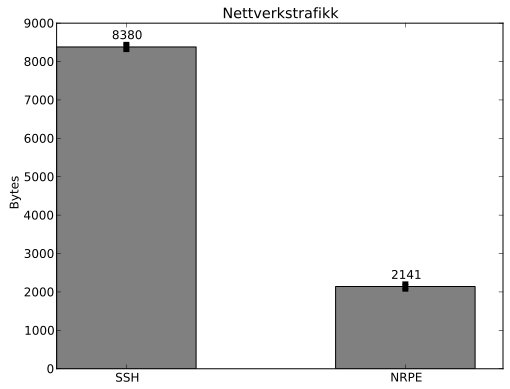
\includegraphics{img/network-usage.svg}
    \caption{Nettverksbruk}
    \label{network-usage}
\end{figure}
\end{center}


\begin{center}
\begin{figure}
    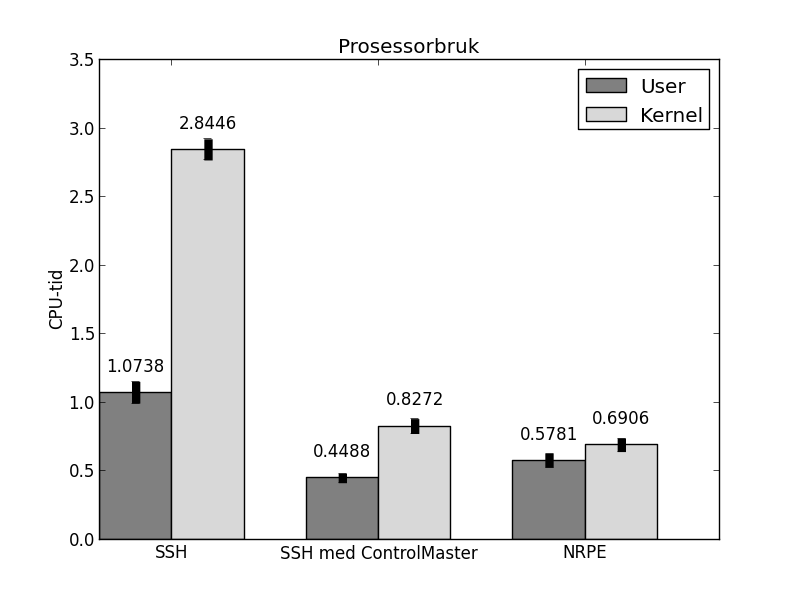
\includegraphics{img/cpu_usage.png}
    \caption{CPU bruk}
    \label{cpu_usage}
\end{figure}
\end{center}


\begin{table}
    \begin{center}
	\begin{threeparttable}
    \begin{tabular}{| l | l | l | l |} \hline
	\ & \textbf{CPU-tid i user(s)} & \textbf{CPU-tid i kernel(s)} & \textbf{Nettverkstrafikk (B)} \\ \hline
	SSH & 1.0738 (0.0792) & 2.8446 (0.0771) & 8380 (101.38) \\ \hline
	NRPE & 0.5781 (0.0347) & 0.6906 (0.0495) & 2141 (55.08) \\ \hline
	SSH med ControlMaster & 0.4488 (0.0509) & 0.8272 (0.0543) & 1700* \\ \hline
	\end{tabular}
	\begin{tablenotes}
	\small
	\item *For SSH med ControlMaster var det ikke mulig å sortere ut hvor mye trafikk det var på én sjekk. Her er det brukt et gjennomsnitt ved å dele den totale mengden trafikk på antall sjekker.
	\end{tablenotes}
	\caption{Prosessorforbruk test med agenter}
	\label{agentcheck}
	\end{threeparttable}
	\end{center}
\end{table}

Det ble valgt å benytte NRPE både for Linux- og Windows-servere. En fordel med dette er at det kan benytte samme protokoll for alle tilkoblinger fra Icinga-serveren til samme port (5666) på andre servere. Dette gjør at det kun trengs én brannmurregel for Icinga, som igjen holder antall angrepsvektorer nede. En annen fordel er at samme service- og command-objekter kan benyttes i Icinga for sjekker som skal utføres via NRPE, uavhengig av om hosten kjører Windows eller Linux.


